\documentclass[11pt]{article}
\usepackage[margin=1.0in]{geometry}
\usepackage{mathtools}
\usepackage{graphicx}
\usepackage{float}
\usepackage[font=small]{caption}
\usepackage{color}
\usepackage{fancyhdr}
%\usepackage{soul} %for striking out text
%\usepackage{arydshln} % for dotted line on truth table
\usepackage{tikz} % graphics stuff
\usepackage{caption}
\usepackage{gensymb}
\usepackage{booktabs}
\usepackage{listings}
\usepackage{fancyvrb}
%\usepackage{subcaption} % used to horizontally tile figures
%\usepackage{listings}
\pagestyle{fancy}
\fancyhead{}
\fancyfoot{}
\fancyfoot[R]{\thepage}

\begin{document}

%
% cover page
%

\vspace*{2 cm}

\begin{center}
\bf{CMPE-630 Digital IC Design\\
    Laboratory Exercise 4\\
\vspace{0.25 cm}
Layout of CMOS Logic Gates
}
\end{center}

\vspace{6 cm}

\begin{flushright}
Brandon Key\\
Performed: 25 Sept 2019\\
Submitted: 9 Oct 2019\\
\vspace{0.5 cm}
Instructor: Dr. Amlan Ganguly\\
TAs: Abhishek Vashist\\
Andrew Fountain\\
Piers Kwan\\
\vspace{0.5 cm}
\end{flushright}

\vspace{3 cm}
\indent By submitting this report, you attest that you neither have given nor have received any assistance (including writing, collecting data, plotting figures, tables or graphs, or using previous student reports as a reference), and you further acknowledge that giving or receiving such assistance will result in a failing grade for this course.

\vspace{1 cm}
Your Signature:   \rule{13cm}{.1pt}


\tableofcontents
\newpage

\section{Abstract}
	The layout and performance of a CMOS inverter was explored in this exercise. Pyxis layout tool was used to generate the layout. During the process, the Design Rule Check (DRC) was used to verify that the design is able to be fabricated. Total area of the circuit was: Height = 3.64$\mu$m, Width = 3.25$\mu$m. A parasitic extraction was performed to obtain frequency response of the circuit. The unloaded maximum input frequency was 55Hz,and the throughput of 120Hz. A decrease of 18079\% was the change in input frequency versus the schematic only frequency response. The throughput decreased 20515\% over the schematic timing. 


\section{Design Methodology and Theory}

	Layout is a critical step in integrated circuit design. A layout for a circuit sets the physical materials and sizes used in a circuit. There are many considerations when creating a circuit layout such as performance and power draw. Each of these topics is a complex topic, and this exercise focused mainly on circuit functionality and how it relates to the fabrication process. To keep the design simple, the inverter from Exercise 2 was laid out. The schematic for the inverter can be seen in Figure \ref{fig:inverter-schematic}.

	\begin{figure}[H]
		\centering
		\includegraphics[width=0.7\linewidth]{"Pictures/Inverter Schematic"}
		\caption{Inverter Schematic}
		\label{fig:inverter-schematic}
	\end{figure}

	A stick diagram is a quick way to get a rough idea about how a layout will look. A typical circuit will have a ground and $V_{dd}$ rail on the bottom and top of the diagram respectively. These rails allows different gates to be constructed within the same vertical space and it simplifies the layout. These rails also allow easy routing of power across a chip. Another common design pattern is having a P-run and and N-Run right within the power rails. This shortens the source connections and again, simplifies design. Having relatively uniform layout increases the chance that fabrication will be successful, as well as simplifying the design. With these considerations, the stick diagram in Figure \ref{fig:stick-diagram}. 

	\begin{figure}[H]
		\centering
		\includegraphics[width=0.7\linewidth]{"Pictures/Stick Diagram"}
		\caption{Stick Diagram for Inverter}
		\label{fig:stick-diagram}
	\end{figure}
	
	
	
	\subsection{Design Rules}
		
		Design rules are set by a foundry and are based off of the process used. Design rules help ensure that a layout is physically possible to make and would function as expected. While a layout does not show it, the process of applying masks and etching does not create perfectly straight or aligned edges. This non-exact process means that parts of a design need space between them, or need a min/max size. Other design rules ensure that a circuit will function as expected. One such example is requiring a P-Well to have a N-Well within a maximum distance so that the body of the transistor is tied to Vdd. Without the connection, the body will be floating and a channel may form when it is not intentional. 
	
	\subsection{Layers}
	
		\subsubsection{OD - Open Diffusion}
		This the channel region of the transistor. The doping in this region determines the voltage levels of the transistor and allows a controlled place for current flow.
		
		\subsubsection{POLYG - Polysilicon Gate}
		Polysilicon is one of the first layers placed in a fabrication process. It has high heat resistance which makes it tolerable to future fabrication stages. The high heat resistance of the polysilicon allows the two side of a transistor to be automatically aligned, since the polysilicon acts as a mask between the two sides. The polysilicon makes a good connection with depletion regions, which makes it excellent for a gate material. The downside of polysilicon is the high resistance, which would make it problematic for current flow, but a gate should not have any current flow. 
		
		\subsubsection{PP - P Pick}
		Forms a P-doped region. This in combination with a open diffusion region forms what is the P-run in the stick diagram. The P Pick must lie within an N-Well to form a diode barrier. Without this diode barrier, current will flow between the channel and the body of the transistor. 
		
		\subsubsection{NP - N Pick}
		Forms an N-doped region. The open diffusion region will be placed inside the N Pick to form the channel.
		
		\subsubsection{PW - P Well}
		A P Well s a P-doped region that separates the N Pick form the substrate, which forms a diode barrier, thus prevent unwanted body-channel current flow. 
		
		\subsubsection{NW - N Well}
		An N Well is an N-doped region that separates the P Pick from the substrate, which prevents current flow by forming diodes. 
		
		\subsubsection{CO - Contact}
		Contacts connect different layers. In general, more contacts is better as it decreases resistance, thus increasing current flow. 
		
		\subsubsection{M1 - Metal 1}
		Metal is used for connecting different parts of the circuit. It is one of the later stages to be fabricated due to the low melting point of metal. Metal is a highly conductive, but capacitive material. It is ideal for connecting components, but the side should be kept to a minimum or the capacitance increases. Multiple layers of metal can be used, but cost and complexity are increased when this is done.
		

\section{Results and Analysis}

	The layout in this exercise was based off of the stick diagram and the sizing was determine by the Design Rules. The final layout could have been much more efficient, but most of this exercise was learning the Pyxis Layout tool. The Layout was verified using a Design Rule Check (DRC). The verified design was then compared to the schematic with a Layout Versus Schematic (LVS). A spice file was then created of the circuit. It was used to perform a Parasitic Extraction (PEX) in conjunction with a GDSII file that was generated with Pyxis. Eldo was used to perform a transient simulation and generate a waveform database file (.wdb). The waveform database was then displayed with EZwave where timing measurements were recorded.  

	\subsection{Layout}
	
		There are many ways to layout a circuit, so this circuit was designed such that many circuits could be placed next to each-other. This design pattern shows itself with the continuous runs $V_{DD}$, GROUND, P and N runs. The end result can be seen in Figure \ref{fig:layout}.
		
		\begin{figure}[H]
			\centering
			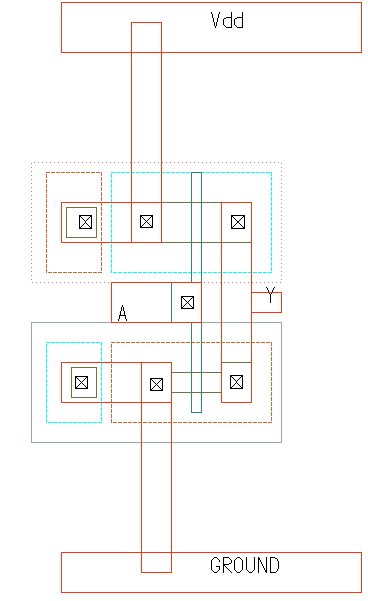
\includegraphics[width=0.7\linewidth]{Pictures/Layout}
			\caption{Inverter Layout}
			\label{fig:layout}
		\end{figure}
	
		The inverter is the smallest circuit that can be made, so vertical space is not very important for this particular circuit as other gates will likely be much taller. Trying to reduce horizontal space was more important so more gates could fit together.

	\subsection {Area}
	
		The inverter is under question in this exercise is the unit inverter so it is the smallest circuit that can be created. This circuit was created with one NMOS and one PMOS. The NMOS was 2$\lambda$ wide, while the PMOS was 4$\lambda$ wide to compensate for the higher internal resistance of PMOS. The length of the transistor was determined by the width of the poly-silicon gate, which was 2$\lambda$. The size of the contacts were set by the Design Rule to 0.16$\mu$m The sizes of wells and taps were set to the minimum size allowed by the Design Rules. The metal paths were set to a convenient size. In hind sight, the metal should have been as small as possible to reduce capacitance. The overall size of the inverter can be seen in Figure \ref{fig:area}
		
		\begin{figure}[H]
			\centering
			\includegraphics[width=0.7\linewidth]{"Pictures/Inverter Area"}
			\caption{Inverter Area}
			\label{fig:area}
		\end{figure}
		
		The height of an inverter is almost always non-consequential as more complex circuits will often take more size, none-the-less the height was 3.64$\mu$m. The width of the inverter was 3.25$\mu$m.
	
	\subsection{Timing}
	
		A Parasitic Extraction (PEX) was performed to gain timing results of the circuit. A SPICE file was created to match the layout and schematic. The SPICE file specified the transient simulation parameters as well as the temperature and load capacitance. The transient simulation parameters were as follows:		
		\begin{itemize}
			\item Magnitude: 1.2V
			\item Width: 50nS
			\item Rise Time: 0.1nS
			\item Fall Time: 0.1nS
			\item Period: 100ns
		\end{itemize}
	
		The timing values were extracted for a load capacitance of 0fF and 120fF. The temperature was set to $25\deg C$. The EZview waveform and timing measurements can be seen in Figure \ref{fig:nominal-no-cap}.
		
		\begin{figure}[H]
			\centering
			\includegraphics[width=0.7\linewidth]{"Pictures/Nominal No Cap"}
			\caption{Nominal Timing; No Load; Temp = 25$\deg$C; $V_{dd}$ = 1.2V}
			\label{fig:nominal-no-cap}
		\end{figure}
	
		The timing results of the circuit were recorded in Figure \ref{fig:measured-timing-results}.
	
		The timing was repeated with a load capacitance of 120fF. The outcome of the simulation were captured in Figure \ref{fig:nominal-cap}.
		
		\begin{figure}[H]
			\centering
			\includegraphics[width=0.7\linewidth]{"Pictures/Nominal Cap"}
			\caption{Nominal Timing; Load = 120fF; Temp = 25$\deg$C; $V_{dd}$ = 1.2V}
			\label{fig:nominal-cap}
		\end{figure}
	
		Adding the load capacitor has must less effect on the timing compared to circuits in the past. This is likely due to the significantly worse performance of this circuit.
	
		The timing measurement was repeated for a worst case scenario, where the voltage was reduced to 1.08V and the temperature was raised to $125\deg C$. The resulting simulation can be seen in Figure \ref{fig:worst-case-no-cap}.
		
		\begin{figure}[H]
			\centering
			\includegraphics[width=0.7\linewidth]{"Pictures/Worst Case No Cap"}
			\caption{Worst Case Timing; No Load; Temp = 125$\deg$C; $V_{dd}$ = 1.08V}
			\label{fig:worst-case-no-cap}
		\end{figure}
	
		The temperature and voltage change decreased performance by around 20\% across the board.
		
		
		Again, a load capacitor was added to the circuit and recorded in Figure \ref{fig:worst-case-cap}.
		
		\begin{figure}[H]
			\centering
			\includegraphics[width=0.7\linewidth]{"Pictures/Worst Case Cap"}
			\caption{Worst Case Timing; Load = 120fF; Temp = 125$\deg$C; $V_{dd}$ = 1.08V}
			\label{fig:worst-case-cap}
		\end{figure}

		Adding the capacitor decreased performance by 10-15\%.
		
		The layout that was created was compared to the assumed performance without layout. The resulting comparison can be seen in Figure \ref{fig:measured-timing-results}.

		
		\begin{figure}[H]
			\centering
			\includegraphics[width=0.7\linewidth]{"Pictures/Measured Timing Results"}
			\caption{Measured Timing Results}
			\label{fig:measured-timing-results}
		\end{figure}
	
		The layout was many times slower than the assumed design. There are many optimizations that could be applied to the circuit such as thinner metal spacing, and more contacts. The largest contributing factor to the slow down is that the parameters for the simulation were not correct. The parasitic capacitance was improperly in the PEX file. It should have been UNIT CAPACITANCE fF instead of UNIT CAPACITANCE pF.
		
		The frequency response of the system was determined with Equation \ref{eqn:Finputmax} and Equation \ref{eqn:Fthroughputmax}. The results of the timing calculations were recorded in \ref{fig:frequency-response-results}. 
	
	
		\begin{equation}\label{eqn:Finputmax}
		F_{input,max} = \frac{1}{t_{rise}+t_{fall}}
		\end{equation}
		\begin{center}
			Equation \ref{eqn:Finputmax}: Max Input Frequency
		\end{center}
		
		\begin{equation}\label{eqn:Fthroughputmax}
		F_{throughput,max} = \frac{1}{T_{P,HL}+T_{P,LH}}
		\end{equation}
		\begin{center}
			Equation \ref{eqn:Fthroughputmax}: Max Throughput Frequency 
		\end{center}
		
		\begin{figure}[H]
			\centering
			\includegraphics[width=0.7\linewidth]{"Pictures/Frequency Response Results"}
			\caption{Frequency Response Results}
			\label{fig:frequency-response-results}
		\end{figure}
	
		The frequency was significantly decreased because of the incorrect simulation parameters.

\clearpage
\vfill
\section{Conclusion}
	This inverter has terrible timing. Some improvements that could be made are increasing the number of contacts between metal and depletion regions. The width of metal could also be reduced to decrease capacitance. The inverter functions as designs, which was the main goal of the exercise. The frustrating process of layout was learned mostly through trial and error, where errors came from the DRC. It was learned that the performance of a circuit is a highly complex subject with many parameters. 


\section*{Questions}
	\textbf{From your extracted SPICE netlist, draw a picture of your inverter with the extracted parasitic capacitances and resistances.  You will need the files that are included in your .sp file (.include $<$filename$>$).  Briefly discuss what each RC network represents}
	
	The sub-circuit PM\_INV\_VDD represents the network around VDD. The sub-circuit PM\_INV\_GROUND represents the network around ground. The sub-circuit PM\_INV\_Y represents the network around the output. The sub-circuit PM\_INV\_A represents the network around the input. 
	
	\begin{figure}[H]
		\centering
		\includegraphics[width=1\linewidth]{"Pictures/Parasidic Caps"}
		\caption{Parasitic Capacitance}
		\label{fig:parasidic-caps}
	\end{figure}


\section{Apendix}

	\begin{lstlisting}
		* File: inv.pex.netlist.pex
		* Created: Sat Oct  5 12:06:08 2019
		* Program "Calibre xRC"
		* Version "v2013.4_26.18"
		* Nominal Temperature: 27C
		* Circuit Temperature: 27C
		* 
		.subckt PM_INV_VDD 1 3 16
		c0 20 0 0.313075f
		c1 14 0 0.636775f
		c2 13 0 0.387652f
		c3 12 0 0.09308f
		c4 5 0 0.234308f
		r5 14 20 0.0217414
		r6 14 16 0.08
		r7 13 20 0.0211941
		r8 12 18 0.0262258
		r9 12 13 0.4
		r10 5 18 0.0196693
		r11 5 7 0.0906154
		r12 3 22 5.49
		r13 1 22 2.66054
		r14 1 18 15.53
		r15 1 7 15.61
		.ends
		
		.subckt PM_INV_GROUND 1 2 17
		c0 18 0 0.313348f
		c1 15 0 0.565028f
		c2 14 0 0.480732f
		c3 8 0 0.261868f
		r4 15 18 0.0264985
		r5 15 17 0.08
		r6 14 20 0.0262258
		r7 13 18 0.0157129
		r8 13 14 0.4
		r9 8 20 0.0196693
		r10 8 10 0.119077
		r11 2 23 5.13774
		r12 2 20 15.61
		r13 2 10 15.53
		r14 1 23 3.0308
		.ends
		
		.subckt PM_INV_Y 1 3 17
		c0 19 0 0.03094f
		c1 17 0 0.093154f
		c2 12 0 0.263831f
		c3 7 0 0.263831f
		r4 15 19 0.0185957
		r5 15 17 0.06
		r6 10 19 0.0238874
		r7 10 12 0.188923
		r8 5 19 0.0238874
		r9 5 7 0.18441
		r10 4 12 15.53
		r11 4 7 15.61
		r12 3 4 4.575
		r13 1 4 8.26517
		.ends
		
		.subckt PM_INV_A 4 8 12
		c0 15 0 0.31096f
		c1 10 0 0.19656f
		c2 8 0 0.335954f
		c3 4 0 0.277194f
		r4 12 15 0.136923
		r5 10 21 11.2861
		r6 10 19 11.5938
		r7 10 15 11.07
		r8 8 21 60
		r9 4 19 60
		.ends
			
	\end{lstlisting}

\end{document}
